\lecture{20}{May 19.}{}
\section{List-coloring}
Given \(G = (V, E)\), and a set of lists \((L_v: v \in V)\). A proper list-coloring is a proper coloring \(\varphi :V \to \bigcup_{v} L_v \) s.t. \(\forall v\) we have \(\varphi (v) \in L_v\), i.e. we want to satisfy the restriction:
\begin{itemize}
    \item \(\forall v \in V\), \(\varphi (v) \in L_v\). 
    \item \(\forall \left\{ u, v \right\} \in E\), \(\varphi (u) \neq \varphi (v)\).     
\end{itemize}     

\begin{definition}
    A graph \(G\) is \(k\)-choosable (or \(k\)-list-colorable) if for any list assignment \((L_v: v \in V)\) with \(\vert L_v \vert \ge k \), there is a proper list-coloring. The choosability or list-chromatic number is 
    \[
        \chi_{\ell} (G) = \mathrm{ch}(G) = \min \left\{ \ell : G \text{ is } \ell \text{-choosable}   \right\}.  
    \]
\end{definition}

\begin{observation}
    \(G\) is \(k\)-choosable implies \(G\) is \((k + 1)\)-choosable.    
\end{observation}

\begin{remark}
    \(\chi _{\ell} (G) \le \Delta (G) + 1\) via the same greedy coloring algorithm. (In fact, \(\chi _\ell (G) \le \mathrm{degen}(G) + 1 \))  
\end{remark}

\begin{remark}
    \(\chi _\ell (G) \ge \chi (G)\), which is because assigning \(L_v = [k]\) turns list-coloring into \(k\)-coloring.   
\end{remark}

\begin{remark}
    Not clear if deciding if a graph is \(k\)-choosable is in NP or co-NP. 
\end{remark}

\begin{proposition} \label{prop: choosability can be arbitrarily larger than chromatic number}
    \(\chi _\ell (G)\) can be arbitrarily larger than \(\chi (G)\).  
\end{proposition}

\begin{eg}
    For \(K_{2, 2}\), we have 
    \[
        \chi _\ell (K_{2, 2}) = 2 = \chi (K_{2, 2}).
    \] 
    %fig
\end{eg}

\begin{explanation}
    Let \(V(G) = \left\{ a, b \right\} \cup \left\{ c, d \right\}  \). We consider the following two cases. 

    \textbf{Case 1:} \(L_a \cap L_b \neq \varnothing\). 

    Then WLOG suppose \(1 \in L_a \cap L_b\). Then we just choose \(\varphi (a) = \varphi (b) = 1\), and choose \(\varphi (c), \varphi (d) \neq 1\). This gives a proper list-coloring. 

    \textbf{Case 2:} \(L_a \cap L_b = \varnothing \). 

    Then there are 4 different pairs of colors that we can assign to \(a\) and \(b\), so it is always possible to find one such pair and assign adequate \(\varphi (c)\) and \(\varphi (d)\) so that \(\varphi (c)\) and \(\varphi (d)\) are both avoided.              
\end{explanation}

\begin{eg}
    For \(K_{3, 3}\), we need to use at least two colors on each side, so there is a color on both sides, so edge between is monochromatic. Thus,
    \[
        \chi _\ell (K_{3, 3}) \ge 3 > 2 = \chi (K_{3, 3}).
    \] 
    \centering
    \begin{tikzpicture}[
        vertex/.style={circle, draw, fill=white, inner sep=1.5pt, minimum size=20pt},
        edge/.style={draw, thick},
        list/.style={font=\small}
        ]
        \node[vertex] (L1) at (0, 2) {$L_1$};
        \node[vertex] (L2) at (0, 0) {$L_2$};
        \node[vertex] (L3) at (0,-2) {$L_3$};

        \node[vertex] (R1) at (4, 2) {$R_1$};
        \node[vertex] (R2) at (4, 0) {$R_2$};
        \node[vertex] (R3) at (4,-2) {$R_3$};

        \foreach \i in {1,2,3} {
            \foreach \j in {1,2,3} {
            \draw[edge] (L\i) -- (R\j);
            }
        }

        \node[list, left=7pt of L1] {$\{1,2\}$};
        \node[list, left=7pt of L2] {$\{1,3\}$};
        \node[list, left=7pt of L3] {$\{2,3\}$};

        \node[list, right=7pt of R1] {$\{1,2\}$};
        \node[list, right=7pt of R2] {$\{1,3\}$};
        \node[list, right=7pt of R3] {$\{2,3\}$};

        \node[font=\large] at (0, 3) {$L$};
        \node[font=\large] at (4, 3) {$R$};
        \node[font=\large] at (2,-3) {$K_{3,3}=L\cup R$};
    \end{tikzpicture}
\end{eg}

\begin{claim}
    For \(m = \binom{2k - 1}{k}\), \(\chi _\ell (K_{m, m}) > k\), where \(\chi (K_{m, m})= 2\).   
\end{claim}

\begin{explanation}
    Let \([2k - 1]\) be the set of all colors. Then there are \(\binom{2k - 1}{k}\) possible lists of \(k\) colors. We assign each such list to a vertex on each side. In a proper list coloring of \(K_{m, m}\), no color appears on both sides. Thus, we have a partition \([2k - 1] = L \cupdot R\), where \(L\) is the set of left colors and \(R\) is the set of right colors. WLOG, \(\vert L \vert \le k - 1\), then \(\exists v\) in the left with \(L_v \subseteq [2k - 1] \setminus L\) since \([2k - 1] \setminus L\) has \(\ge k\) colors. However, \(\varphi (v) \in L_v\) and \(\varphi (v) \in L\), which is impossible. 

    Thus, 
    \[
        c \log m \thickapprox k < \chi _\ell (K_{m, m}) \le m + 1.
    \]            
\end{explanation}

This claim shows \autoref{prop: choosability can be arbitrarily larger than chromatic number}. 

\section{List-coloring planar graph}
\begin{definition}
    A graph \(G\) is planar if it can be drawn in \(\mathbb{R} ^2\) without crossing edges. 
    %fig  
\end{definition}

\begin{theorem}[Euler]
    If \(G\) is an \(n\)-vertex planar graph, then \(e(G) \le 3n - 6\).   
\end{theorem}

\begin{theorem}[Kuratowski]
    \(G\) is planar iff \(G\) does not contain a subdivision\footnote{Basically, a subdivision of a graph is replacing some edges of the graph by paths - essentially a relaxion of a graph. But this isn't very important in this course, so we won't be formally defining it here.} of \(K_5\) or \(K_{3, 3}\).    
\end{theorem}

\begin{theorem}[Four color theorem]
    If \(G\) is planar, then \(\chi (G) \le 4\).  
\end{theorem}

Before proving this, we can give an oservation.

\begin{observation}
    \(e(G) \le 3 n - 6\) for all planar graph implies \(\mathrm{degen}(G) \le 5\), so \(\chi (G) \le 6\).   
\end{observation}

\begin{proof}
It suffices to show that every subgraph of \(G\) has a vertex of degree at most \(5\).
Let \(H\) be any nonempty subgraph of \(G\), and write \(v(H)=m\) and \(e(H)\) for its number of vertices and edges.
Since every subgraph of a planar graph is planar, \(H\) is planar. If \(m\ge 3\), then
\[
    e(H) \le 3m-6.
\]
Hence the average degree of \(H\) is
\[
    \frac{2e(H)}{m} \le \frac{2(3m-6)}{m} = 6-\frac{12}{m} < 6.
\]
Therefore \(H\) has a vertex of degree at most \(5\). If \(m<3\), this is immediate.
Thus every subgraph of \(G\) contains a vertex of degree at most \(5\), so \(G\) is \(5\)-degenerate.

Finally, every \(d\)-degenerate graph is \((d+1)\)-colorable: order the vertices by repeatedly deleting a vertex of degree at most \(d\), then color them in the reverse order. When a vertex is colored, it has at most \(d\) already-colored neighbors, so one of \(d+1\) colors is available. Applying this with \(d=5\), we get
\[
    \chi(G) \le 6.
\]
\end{proof}

\begin{theorem}[Heawood, 1890]
    If \(G\) is planar, then \(\chi (G) \le 5\).  
\end{theorem}
\begin{proof}
    Graph Theory I. 
\end{proof}

\begin{theorem}[Appel-Haken, 1976]
    If \(G\) is planar, \(\chi (G) \le 4\).   
\end{theorem}

\begin{remark}
    This is the first significant computer-aided proof. Subsequently simplified by Robertson, Seymour, Thomas.
\end{remark}

\begin{proposition}[Mirzakhani, Voigt]
    There is a planar graph \(G\) that is not 4-choosable. 
\end{proposition}
\begin{proof}
    HW.
\end{proof}

\begin{theorem}[Thomassen]
    If \(G\) is planar, then \(\chi _\ell (G) \le 5\).  
\end{theorem}

\begin{proof}
    We may assume 
    \begin{itemize}
        \item The outer face of \(G\) is a cycle with vertices \(v_1, v_2, \dots , v_{\ell} \) in a cyclic order. 
        \item Every bounded face of \(G\) is a triangle. (since we can triangulating the larger cycles). 
    \end{itemize}
    We can give a stronger claim: We can find a proper coloring from lists \((L_v: v \in V)\) where 
    \begin{itemize}
        \item \(\vert L_{v_1} \vert = \vert L_{v_2} \vert = 1, L_{v_1} \neq L_{v_2}\). 
        \item \(\vert L_{v_i} \vert \ge 3, \quad \forall 3 \le i \le \ell \). 
        \item \(\vert L_v \vert \ge 5 \) for all internal \(v\).    
    \end{itemize} 
    Now we can prove by induction on \(\vert V(G) \vert \). 

    Base case: \(\vert V(G) \vert = 3\), so \(G = K_3\), then since \(\vert L_{v_3} \vert \ge 3 \), \(L_{v_3} \setminus (L_{v_1} \cup L_{v_2}) \neq \varnothing\), and thus we can find color for \(v_3\) distinct from those of \(v_1\) and \(v_2\). 

    Induction step: 

    \textbf{Case 1:} There is a chord \(\left\{ v_i, v_j \right\} \in E(G) \) where \(\vert j - i \vert \ge 2 \mod{\ell}\). This splits the graph into two: 
    \begin{itemize}
        \item \(G_1\): boundary \(v_1, v_2, \dots , v_i, v_j, v_{j+1}, \dots , v_{\ell}\). 
        \item \(G_2\): boundary \(v_i, v_{i+1}, v_{i+2}, \dots , v_{j-1}, v_j\).    
    \end{itemize}       
    By induction, we can color \(G_1\). In \(G_2\), restrict the lists of \(v_i, v_j\) to the colors they receive in \(G_1\). All other boundary vertices still have lists of size 3, internal vertices hace lists of size 5. By induction (with \(v_i, v_j\) playing the role of \(v_1, v_2\)), we can color \(G_2\), and we can combine them to get a coloring of \(G\). 

    \textbf{Case 2: the outer cycle has no chord.} We remove $v_3$. Since every
    bounded face is a triangle and there are no chords of the outer cycle, the
    neighbors of $v_3$ are
    \[
        v_2, u_1,u_2,\ldots,u_m, v_4,
    \]
    in order around $v_3$, where the $u_k$ are internal vertices of $G$. After
    deleting $v_3$, those internal neighbors become part of the new outer face.
    \vspace{-4em}
    \begin{center}
    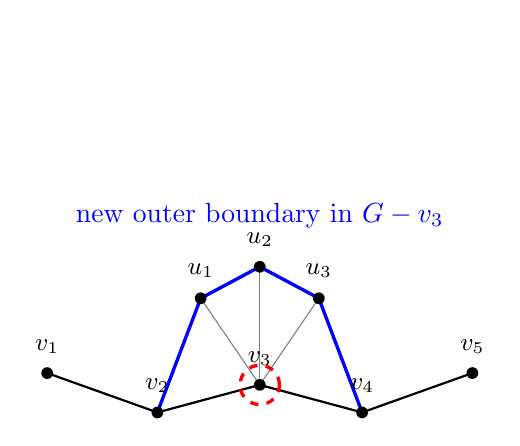
\begin{tikzpicture}[scale=1, every node/.style={circle, fill=black, inner sep=1.5pt}]
        \coordinate (v1) at (-2.7,-1.1);
        \coordinate (v2) at (-1.3,-1.6);
        \coordinate (v3) at (0,-1.25);
        \coordinate (v4) at (1.3,-1.6);
        \coordinate (v5) at (2.7,-1.1);
        \coordinate (u1) at (-0.75,-0.15);
        \coordinate (u2) at (0,0.25);
        \coordinate (u3) at (0.75,-0.15);
        \draw[thick] (v1) -- (v2) -- (v3) -- (v4) -- (v5);
        \draw[thick] (v2) -- (u1) -- (u2) -- (u3) -- (v4);
        \draw[gray] (v3) -- (u1);
        \draw[gray] (v3) -- (u2);
        \draw[gray] (v3) -- (u3);
        \draw[gray] (v2) -- (u1);
        \draw[gray] (u1) -- (u2);
        \draw[gray] (u2) -- (u3);
        \draw[gray] (u3) -- (v4);
        \draw[very thick, dashed, red] (v3) circle[radius=0.25];
        \draw[blue, very thick] (v2) -- (u1) -- (u2) -- (u3) -- (v4);
        \foreach \p/\name in {v1/$v_1$,v2/$v_2$,v3/$v_3$,v4/$v_4$,v5/$v_5$,u1/$u_1$,u2/$u_2$,u3/$u_3$}
            \node[label={[font=\small]\name}] at (\p) {};
        \node[draw=none, fill=none, text=blue] at (0,0.9) {new outer boundary in $G-v_3$};
    \end{tikzpicture}
    \end{center}
    \vspace{2em}

    Choose two distinct colors
    \[
        x,y\in L_{v_3}\setminus L_{v_2}.
    \]
    This is possible because $|L_{v_3}|\ge 3$ and $L_{v_2}$ contains only one color.
    For each internal neighbor $u_k$ of $v_3$, delete the colors $x$ and $y$ from
    $L_{u_k}$. Each $u_k$ originally had at least $5$ colors, so after deleting at
    most two colors it still has at least $3$ colors. Thus, in $G-v_3$, the newly
    exposed boundary vertices $u_k$ satisfy the boundary-list condition.

    By induction, $G-v_3$ has a proper list-coloring from these modified lists. Now
    we color $v_3$. The color on $v_2$ is not $x$ or $y$ by construction, and none
    of the internal neighbors $u_k$ uses $x$ or $y$ because those colors were
    deleted from their lists. The only remaining neighbor of $v_3$ that might use
    one of $x$ and $y$ is $v_4$. Since $x$ and $y$ are distinct, at least one of
    them is different from the color on $v_4$. Assign that color to $v_3$.

    This gives a proper list-coloring of $G$, completing the induction and hence
    the proof of the theorem.                       

    This finishes the proof of the claim, which then implies the theoem.
\end{proof}